\documentclass[11pt]{book}
 
\newcommand{\reporttitle}{Coupling / Curtains}
\newcommand{\reportauthor}{CARIOU KOTLAREK}
\newcommand{\course}{Semester Paper}
\newcommand{\professor}{JACQUIER ; ACCIAIO}
% include file with configuration.
\input{../config/config_article} % various packages needed for maths etc.



\begin{document}

% neuron circle
\tikzset{%
  every neuron/.style={
    circle,
    draw,
    minimum size=1cm
  },
  neuron missing/.style={
    draw=none, 
    scale=4,
    text height=0.2cm,
    execute at begin node=\color{black}$\vdots$
  },
}

\begin{figure}
\centering
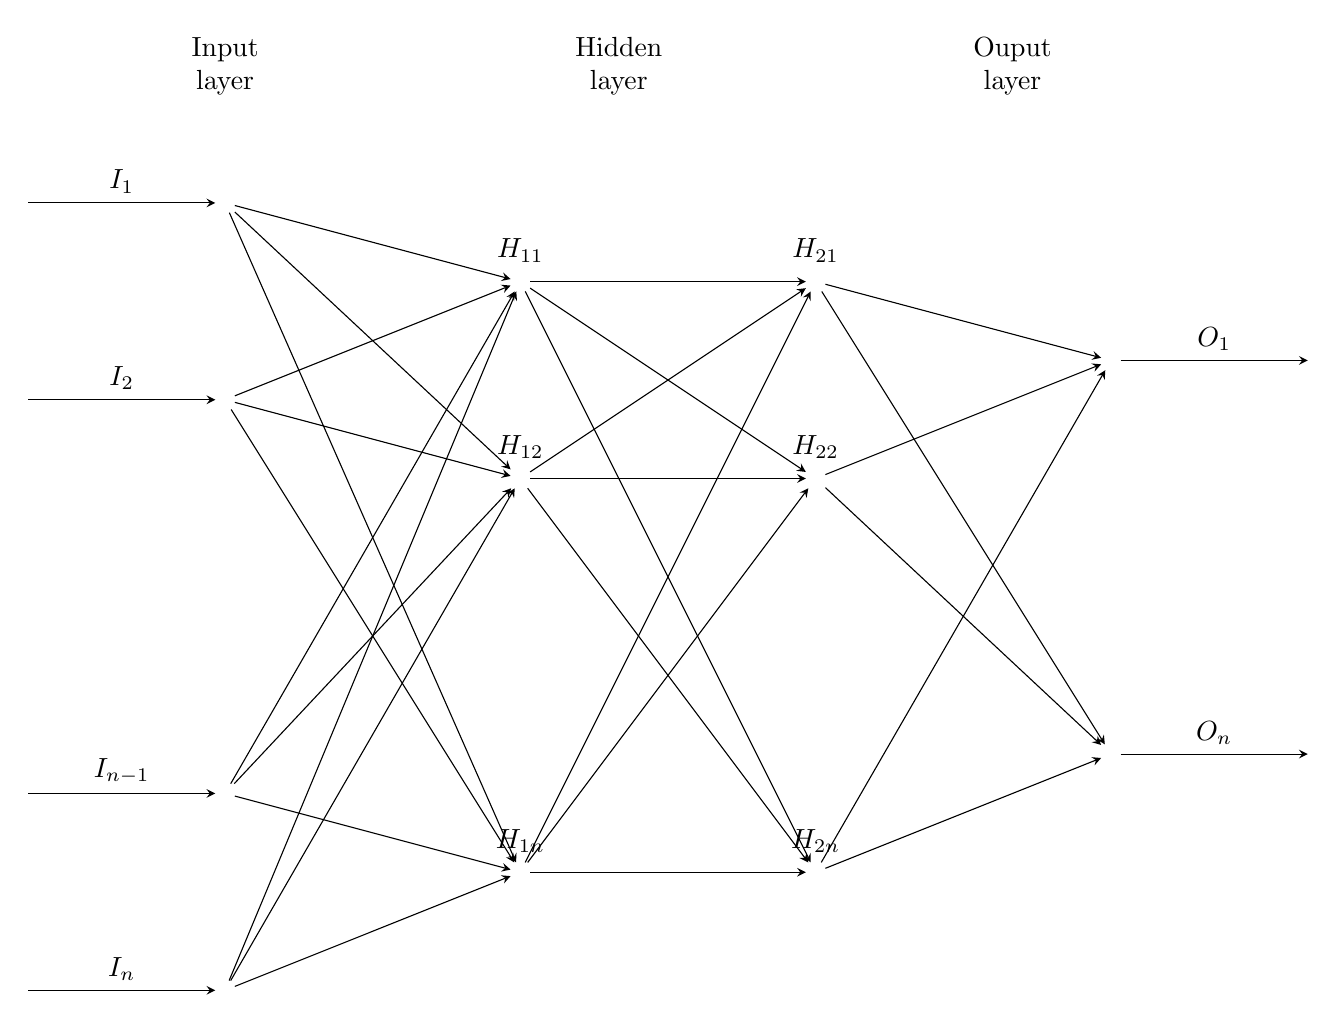
\begin{tikzpicture}[x=2.5cm, y=2.5cm, >=stealth]

% define input layer
\foreach \m/\l [count=\y] in {1,2,missing,3,4}
  \node [every neuron/.try, neuron \m/.try] (input-\m) at (0,2.5-\y) {};

% define hidden layers
\foreach \m [count=\y] in {1,2,missing,3}
  \node [every neuron/.try, neuron \m/.try ] (hiddenOne-\m) at (1.5,2.1-\y) {};

\foreach \m [count=\y] in {1,2,missing,3}
  \node [every neuron/.try, neuron \m/.try ] (hiddenTwo-\m) at (3,2.1-\y) {};
  
% define output layer
\foreach \m [count=\y] in {1,missing,2}
  \node [every neuron/.try, neuron \m/.try ] (output-\m) at (4.5,1.7-\y) {};

% draw input neurons
\foreach \l [count=\i] in {1,2,n-1,n}
  \draw [<-] (input-\i) -- ++(-1,0)
    node [above, midway] {$I_{\l}$};

% draw hidden neurons
\foreach \l [count=\i] in {1,2,n}
  \node [above] at (hiddenOne-\i.north) {$H_{1\l}$};

\foreach \l [count=\i] in {1,2,n}
  \node [above] at (hiddenTwo-\i.north) {$H_{2\l}$};
  
% draw output neurons
\foreach \l [count=\i] in {1,n}
  \draw [->] (output-\i) -- ++(1,0)
    node [above, midway] {$O_\l$};

% connect input neurons to hidden neurons
\foreach \i in {1,...,4}
  \foreach \j in {1,...,3}
    \draw [->] (input-\i) -- (hiddenOne-\j);

% connect hidden neurons to hidden neurons
\foreach \i in {1,...,3}
  \foreach \j in {1,...,3}
    \draw [->] (hiddenOne-\i) -- (hiddenTwo-\j);

% connect hidden neurons to output neurons
\foreach \i in {1,...,3}
  \foreach \j in {1,...,2}
    \draw [->] (hiddenTwo-\i) -- (output-\j);

\foreach \l [count=\x from 0] in {Input, Hidden, Ouput}
  \node [align=center, above] at (\x*2,2) {\l \\ layer};

\end{tikzpicture}
\caption{NN Architecture}
\end{figure}
	


\end{document}